\documentclass[UTF8]{article}
\usepackage{ctex}
\usepackage{verbatim}
%\usepackage{amsmath}
\usepackage{graphicx}
\usepackage{palatino}
\usepackage{tikz}
\usetikzlibrary{shapes.geometric, arrows}

\title{\heiti 电机基础及控制技术}
\author{\heiti 庄梓伸}
\date{\heiti \today}

\begin{document}
\maketitle

\section{前言}
    在机器人领域，电机好比人类的肌肉，没有电机的机器人就是一个摆设，在一个机器人项目中需要选择什么类型的电机，是第一大问题。
    对于初学者而言，在依靠各种参数选型一个电机时，免不了要了解这一类型的电机的构成。
    了解了其构成后，我们项目的关键来到了：如何驱动一个电机？
    这就引出了我们的电机驱动器，电机驱动器就好比人类用于控制肌肉的神经，好的驱动器能够带来电机控制的精度，
    从而增强一个机器人自身的稳定性。本文将从电机的不同种类开始叙述，然后分别展开叙述不同种类电机的组成以及驱动方式。

\newpage

\section{电机分类}

    \begin{figure}[ht]
        \centering
        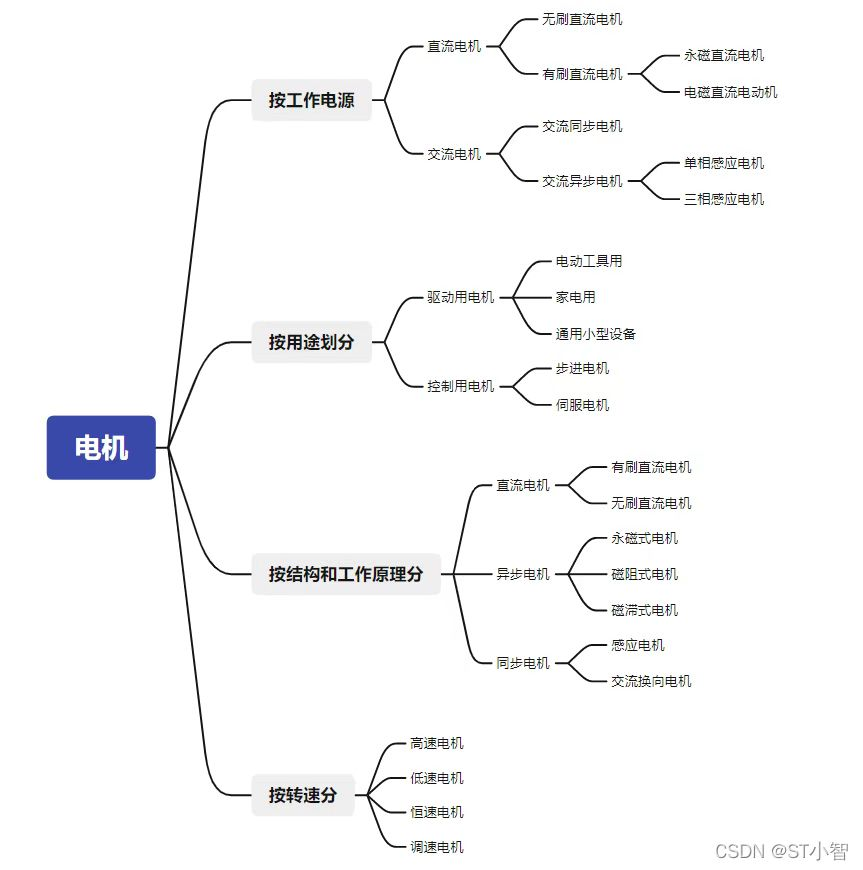
\includegraphics[scale=0.3]{Pic/电机分类.jpg}
    \end{figure}

\end{document}